\documentclass[UTF8]{ctexart}
\usepackage{geometry}
\usepackage{graphicx}
\usepackage{hyperref}
\usepackage{booktabs}
\usepackage{listings}
\usepackage{amsmath}
\usepackage{tikz}
\usetikzlibrary{shapes, arrows, positioning}
\usepackage{amssymb}
\usepackage{xcolor}
\usepackage{fontspec}
\usepackage{titlesec}
\usepackage{float}
\usepackage{subcaption}
\geometry{a4paper, left=2cm, right=2cm, top=2.5cm, bottom=2.5cm}

\definecolor{codegreen}{rgb}{0,0.6,0}
\definecolor{codegray}{rgb}{0.5,0.5,0.5}
\definecolor{codepurple}{rgb}{0.58,0,0.82}
\definecolor{backcolour}{rgb}{0.95,0.95,0.92}

\lstdefinestyle{mystyle}{
    backgroundcolor=\color{backcolour},   
    commentstyle=\color{codegreen},
    keywordstyle=\color{magenta},
    numberstyle=\tiny\color{codegray},
    stringstyle=\color{codepurple},
    basicstyle=\ttfamily\footnotesize,
    breakatwhitespace=false,         
    breaklines=true,                 
    captionpos=b,                    
    keepspaces=true,                 
    numbers=left,                    
    numbersep=5pt,                  
    showspaces=false,                
    showstringspaces=false,
    showtabs=false,                  
    tabsize=2
}

\lstset{style=mystyle}
\begin{document}

\title{C++程序课程设计:五子棋游戏}
\author{24-1班 第2组}
\date{2025年6月11日}

\maketitle
\begin{center}
    \begin{tabular}{|c|c|c|c|}
        \hline
        \textbf{学号} & \textbf{姓名}  \\
        \hline
        2410120028 & Gazettm \\
        \hline
        2410120036 & pajiii \\
        \hline
    \end{tabular}
\end{center}

\tableofcontents
\newpage

\section{程序说明}
本程序是一个基于Qt框架的五子棋游戏,支持人机对战和双人对战两种模式。主要功能包括:
\begin{itemize}
    \item 15×15标准五子棋棋盘
    \item 智能AI对手(防守优先策略)
    \item 胜负判定与游戏结束处理
    \item 胜率统计系统
    \item 美观的图形界面(棋子渐变效果、悬停提示)
    \item 游戏模式选择(人机对战/双人对战)
    \item 悔棋记录功能
\end{itemize}

程序采用面向对象设计,核心类包括GomokuBoard(棋盘逻辑)、AiPlayer(AI算法)、GameWindow(游戏界面)和Rating(胜率统计)。

\section{程序分析}
\subsection{需求分析}
\begin{itemize}
    \item \textbf{功能需求}:实现五子棋基本规则、AI对战、胜负判定、历史胜率统计、悔棋
    \item \textbf{性能需求}:AI响应时间<500ms,界面刷新流畅
    \item \textbf{用户体验}:直观的棋盘布局、棋子悬停提示、游戏状态反馈
\end{itemize}

\subsection{设计挑战}
\begin{itemize}
    \item AI算法需平衡进攻与防守
    \item 实现高效的五子连珠检测
    \item 保证界面响应性与美观性
    \item 胜率数据的持久化存储
    \item 记录棋盘数据用于悔棋
\end{itemize}

\section{程序设计}
\subsection{系统架构}

\subsubsection{逻辑结构图}
\begin{figure}[H]
\centering
\begin{tikzpicture}[
    class/.style={rectangle, draw, rounded corners, minimum width=3cm, align=center, font=\small},
    inherit/.style={->, >=open triangle 60, shorten >=2pt},
    compose/.style={->, >=diamond, shorten >=2pt},
    node distance=2cm
]

% 定义类节点
\node[class] (GameWindow) {GameWindow\nodepart{lower}界面控制\\游戏流程};
\node[class, below=of GameWindow] (GomokuBoard) {GomokuBoard\nodepart{lower}棋盘数据\\胜负判定};
\node[class, right=of GomokuBoard] (AiPlayer) {AiPlayer\nodepart{lower}AI决策\\评分算法};
\node[class, left=of GomokuBoard] (Rating) {Rating\nodepart{lower}胜率统计\\数据持久化};

% 绘制关系箭头
\draw[compose] (GameWindow) -- node[right] {持有} (GomokuBoard);
\draw[compose] (GameWindow) -| node[pos=0.25, above] {人机模式时} (AiPlayer);
\draw[compose] (GameWindow) -| node[pos=0.25, above] {记录战绩} (Rating);
\draw[->, dashed] (AiPlayer) -- node[pos=0.5,below] {读取棋盘状态} (GomokuBoard);

\end{tikzpicture}
\caption{五子棋游戏逻辑结构图}
\label{fig:class-structure}
\end{figure}
\subsubsection{数据流图}
\begin{figure}[H]
\centering
\begin{tikzpicture}[
    process/.style={rectangle, draw, minimum width=4cm, align=center, font=\small},
    decision/.style={diamond, draw, aspect=2, align=center},
    data/.style={ellipse, draw, dashed},
    arrow/.style={->, >=stealth', shorten >=2pt},
    node distance=1cm and 2cm
]

% 定义节点
\node[process] (start) {游戏初始化};
\node[process, below=of start] (wait) {等待玩家落子};
\node[decision, below=of wait] (valid) {落子有效?};
\node[process, right=of valid] (ai) {AI计算落子};
\node[decision, below=of valid,font=\small] (win) {五连判定};
\node[process, left=of win] (end) {显示胜负\\更新胜率};
\node[data, right=of win] (board) {棋盘状态};

% 绘制箭头
\draw[arrow] (start) -- (wait);
\draw[arrow] (wait) -- (valid);
\draw[arrow] (valid) -- node[above] {否} (ai);
\draw[arrow] (ai) |- (wait);
\draw[arrow] (valid) -- node[left] {是} (win);
\draw[arrow] (win) -- node[above] {达成} (end);
\draw[arrow] (win) -| node[pos=0.15, below,font=\small] {未达成} (wait);
\draw[<->, dashed] (board) -- (win);
\draw[<->, dashed] (board) |- (ai);

% 添加图例
\node[anchor=north west] at (current bounding box.north west) {
    \begin{tabular}{@{}ll@{}}
        \tikz\draw[->, >=stealth'] (0,0) -- (0.5,0); & 控制流 \\
        \tikz\draw[<->, dashed] (0,0) -- (0.5,0); & 数据交互 \\
    \end{tabular}
};

\end{tikzpicture}
\caption{五子棋游戏数据流图}
\label{fig:data-flow}
\end{figure}

\subsection{核心类设计}
\begin{itemize}
    \item \textbf{GomokuBoard}:棋盘状态管理、落子逻辑、胜负判定
    \item \textbf{AiPlayer}:位置评估算法、最优落子点计算
    \item \textbf{GameWindow}:界面绘制、事件处理、游戏流程控制
    \item \textbf{Rating}:胜率计算、数据持久化
\end{itemize}
\subsection{AI评估算法}
采用基于规则的评估函数,考虑因素:
\begin{enumerate}
    \item \textbf{防守优先级}:优先阻断对手四连(100000分)
    \item \textbf{进攻机会}:构建自身连珠(优先构建五连999999分)
    \item \textbf{位置价值}:中心区域权重更高
\end{enumerate}

评分权重矩阵:
\[
\text{Score} = \sum_{\text{方向}} \begin{cases} 
100000 & \text{对手4连} \\
10000 & \text{对手活3} \\
5000 & \text{AI活3/4连} \\
500 & \text{AI活2}
\end{cases} + 10 \times (n - |x - c| - |y - c|)
\]

\subsection{胜率统计算法}
\[
\text{胜率} = \frac{Y}{Y + N} \times 100\%
\]
\begin{itemize}
    \item $Y$:从Rating.txt读取的"Y"行数
    \item $N$:从Rating.txt读取的"N"行数
\end{itemize}

\section{程序实现}
\subsection{开发环境}
\begin{itemize}
    \item 操作系统:Linux
    \item 编译器:g++
    \item GUI框架:Qt 5.15
    \item 构建工具:Makefile
\end{itemize}
\subsection{使用头文件介绍}
\begin{itemize}
\item QVector:QT中用于生成动态数组的类,可以构建棋盘的基本逻辑。
\item QPoint:QT中提供的一个二维坐标点类,用于生成五子棋中的棋子。
\item QTimer:用于计算AI落子时间并控制在500ms以内。
\item Qpainter:QT的绘图工具类,用于绘制棋盘,棋子,悬停提示,实现颜色渐变和抗锯齿效果。
\item Qpixmap:QT的图片导入类,用于设置棋盘背景图片。
\item QMouseEvent:处理鼠标的移动,悬停,以及点击事件。
\item QMessageBox:弹出消息提示框,比如选择游戏模式。
\item QElapsedTimer:Qt的高精度计时器类。
\item QApplication:QT中应用程序的核心类,实现全局应用程序控制和游戏循环。
\item fstream:文件操作,存储胜负情况计算胜率。
\item QLinearGradient:QT中实现颜色线性渐变的类,增加棋子质感。
\item QKeyEvent:处理键盘输入信号,本项目用于ctrl+z悔棋功能。
\item QRandomGenerator:用于生成范围内随机数,防止预测AI下一步。
\end{itemize}

\subsection{关键实现}
\subsubsection{棋盘绘制}
使用QPainter实现高质量棋盘渲染:
\begin{lstlisting}[language=C++]
void GameWindow::drawBoard(QPainter &painter) {
    painter.fillRect(..., QBrush(QColor(210, 180, 140, 180)));
    for (int i = 0; i < m_board.size(); ++i) {
        painter.drawLine(...);
        painter.drawLine(...);
    }
    painter.drawEllipse(QPoint(x, y), 4, 4);
}
\end{lstlisting}
\subsubsection{UI设计及键鼠交互}
gamewindow.h
\begin{lstlisting}[language=C++]
#ifndef GAME_WINDOW_H
#define GAME_WINDOW_H

#include <QMainWindow>
#include <QMouseEvent>
#include <QMessageBox>
#include "gomokuboard.h"
#include "aiplayer.h"
#include "Rating.h"
#include <QTimer>
#include <QApplication>
#include <QRandomGenerator>
#include <QPixmap>
#include <cmath>

class GameWindow : public QMainWindow {
    Q_OBJECT 

public:
    enum GameMode { HumanVsHuman, HumanVsAI };
    explicit GameWindow(QWidget *parent = nullptr);
    ~GameWindow() override = default;
    void ShowWinner(GomokuBoard::Piece winner);
    void exitGame();
    void WriteRatingY();
    void WriteRatingN();
	void undoLastMove();

protected:
    void paintEvent(QPaintEvent *event) override;
    void mousePressEvent(QMouseEvent *event) override;
    void mouseMoveEvent(QMouseEvent *event) override;
    void leaveEvent(QEvent *event) override;
	void keyPressEvent(QKeyEvent *event) override;

private:
    GomokuBoard m_board;
    GomokuBoard::Piece m_currentPiece;
    GameMode m_gameMode;
    AiPlayer m_aiplayer;
    Rating rating;
    QPoint m_hoverPos;
	bool isAIpending = false;
	
    void drawBoard(QPainter &painter);
    void drawPieces(QPainter &painter);
    void drawHoverIndicator(QPainter &painter);
};

#endif
\end{lstlisting}
gamewindow.cpp
\begin{lstlisting}[language=C++]
#include "gamewindow.h"
#include <QPainter>
#include <QMouseEvent>
#include <QMessageBox>
#include <QElapsedTimer>
#include <QApplication>
#include <fstream>
#include <QLinearGradient>
#include <QRadialGradient>
#include <QKeyEvent> 

GameWindow::GameWindow(QWidget *parent) : 
    QMainWindow(parent),
    m_board(15), 
    m_currentPiece(GomokuBoard::Black), 
    m_hoverPos(-1, -1) {
    setWindowTitle("Gomoku Game");
    setFixedSize(640, 640);
    setMouseTracking(true);
    show();
    rating.ShowRating();

    QMessageBox::StandardButton reply = QMessageBox::question(
        this,
        "游戏模式 ",
        "Ctrl+z可以悔棋\n请选择游戏模式:\n是 - 人机对战\n否 - 双人对战",
        QMessageBox::Yes | QMessageBox::No
    );
    m_gameMode = (reply == QMessageBox::Yes) ? HumanVsAI : HumanVsHuman;
    
}
void GameWindow::ShowWinner(GomokuBoard::Piece winner) {
    update();
    if (winner == GomokuBoard::Black) {
        if(m_gameMode == HumanVsAI){
            WriteRatingY();
        }

        QMessageBox msgBox;
        msgBox.setText("黑棋获胜!");
        msgBox.setInformativeText("点击确定退出游戏");
        msgBox.setStandardButtons(QMessageBox::Ok);
        msgBox.setDefaultButton(QMessageBox::Ok);

        connect(&msgBox, &QMessageBox::finished, this, &GameWindow::exitGame);

        msgBox.exec();
       } else if (winner == GomokuBoard::White) {
        if(m_gameMode == HumanVsAI){
            WriteRatingN();
        }

        QMessageBox msgBox;
        msgBox.setText("白棋获胜!");
        msgBox.setInformativeText("点击确定退出游戏");
        msgBox.setStandardButtons(QMessageBox::Ok);
        msgBox.setDefaultButton(QMessageBox::Ok);

        connect(&msgBox, &QMessageBox::finished, this, &GameWindow::exitGame);

        msgBox.exec(); 
    }
}
void GameWindow::paintEvent(QPaintEvent *event) {
    QPainter painter(this); 
    painter.setRenderHint(QPainter::Antialiasing);
    painter.drawPixmap(rect(), QPixmap("baka.png"));
    drawBoard(painter);
    drawPieces(painter);
    drawHoverIndicator(painter);
}
void GameWindow::mousePressEvent(QMouseEvent *event) {
    if (m_gameMode == HumanVsAI && m_currentPiece != GomokuBoard::Black) {
        return;
    }

    int gridSize = width() / (m_board.size() + 1);
    int margin = gridSize;
    
    int x = qRound(static_cast<float>(event->x() - margin) / gridSize);
    int y = qRound(static_cast<float>(event->y() - margin) / gridSize);

  if (x < 0 || x >= m_board.size() || y < 0 || y >= m_board.size()) {
        return;
    }

    if (m_board.placePiece(x, y, m_currentPiece)) {
        if (m_board.checkWin(x, y)) {
            ShowWinner(m_currentPiece);
        } else {

            if (m_gameMode == HumanVsAI) {
				isAIpending = true;
                m_currentPiece = GomokuBoard::White;
				
                QTimer::singleShot(500, this, [this]() { 
					
                    QPoint aiMove = m_aiplayer.calculateAIMove(m_board);
                    if (aiMove.x() != -1) {
                        m_board.placePiece(aiMove.x(), aiMove.y(), GomokuBoard::White);
                        if (m_board.checkWin(aiMove.x(), aiMove.y())) {
                            ShowWinner(GomokuBoard::White);
                        } else {
                            m_currentPiece = GomokuBoard::Black;
                        }
                        update();
                        isAIpending = false;
                    }
                });	
            } else {
                m_currentPiece = (m_currentPiece == GomokuBoard::Black) ? GomokuBoard::White : GomokuBoard::Black;
            }
            update();
        }
    }
}

void GameWindow::mouseMoveEvent(QMouseEvent *event) {
    int gridSize = width() / (m_board.size() + 1);
    int margin = gridSize;

    int x = qRound(static_cast<float>(event->x() - margin) / gridSize);
    int y = qRound(static_cast<float>(event->y() - margin) / gridSize);

    if (x >= 0 && x < m_board.size() && 
        y >= 0 && y < m_board.size() && 
        m_board.pieceAt(x, y) == GomokuBoard::Empty) {

        if (m_hoverPos != QPoint(x, y)) {
            m_hoverPos = QPoint(x, y);
            update(); 
        }
    } else {

        if (m_hoverPos != QPoint(-1, -1)) {
            m_hoverPos = QPoint(-1, -1);
            update();
        }
    }
}
void GameWindow::leaveEvent(QEvent *event) {
    Q_UNUSED(event);

    if (m_hoverPos != QPoint(-1, -1)) {
        m_hoverPos = QPoint(-1, -1);
        update(); 
    }
}

void GameWindow::keyPressEvent(QKeyEvent *event) {
	if(isAIpending){
		return;
	}
	if (event->key() == Qt::Key_Z && event->modifiers() & Qt::ControlModifier) {
		undoLastMove();
	}
	QMainWindow::keyPressEvent(event);
}

void GameWindow::drawBoard(QPainter &painter) {
    int gridSize = width() / (m_board.size() + 1);
    int margin = gridSize;
    
    int boardPixels = gridSize * (m_board.size() - 1);
    
    painter.fillRect(margin, margin, 
                   boardPixels, 
                   boardPixels, 
                   QBrush(QColor(210, 180, 140, 180))); 

    painter.setPen(QPen(QColor(13, 102, 171, 150), 4));
    painter.drawRect(margin, margin, 
                   boardPixels, 
                   boardPixels);

    painter.setPen(QPen(QColor(0, 0, 0), 1));
    for (int i = 0; i < m_board.size(); ++i) {
        int pos = margin + i * gridSize;

        painter.drawLine(margin, pos, 
                       margin + boardPixels, 
                       pos);

        painter.drawLine(pos, margin, 
                       pos, 
                       margin + boardPixels);
    }

    painter.setBrush(Qt::black);
    int starPoints[5][2] = {
        {3, 3}, {3, 11}, {7, 7}, {11, 3}, {11, 11} 
    };
    
    for (auto &point : starPoints) {
        int x = margin + point[0] * gridSize;
        int y = margin + point[1] * gridSize;
        painter.drawEllipse(QPoint(x, y), 4, 4); 
    }
}
void GameWindow::drawPieces(QPainter &painter) {
    int gridSize = width() / (m_board.size() + 1);
    int margin = gridSize;
    int pieceRadius = gridSize / 2 - 2;

    for (int x = 0; x < m_board.size(); ++x) {
        for (int y = 0; y < m_board.size(); ++y) {
            if (m_board.pieceAt(x, y) != GomokuBoard::Empty) {

                int centerX = margin + x * gridSize;
                int centerY = margin + y * gridSize;
                
                if (m_board.pieceAt(x, y) == GomokuBoard::Black) {

                    QRadialGradient gradient(centerX, centerY, pieceRadius, 
                                           centerX - pieceRadius/3, centerY - pieceRadius/3);
                    gradient.setColorAt(0, QColor(60, 60, 60)); 
                    gradient.setColorAt(1, Qt::black);          
                    painter.setBrush(gradient);
                } else {

                    QRadialGradient gradient(centerX, centerY, pieceRadius, 
                                           centerX - pieceRadius/3, centerY - pieceRadius/3);
                    gradient.setColorAt(0, Qt::white);
                    gradient.setColorAt(1, QColor(220, 220, 220));
                    painter.setBrush(gradient);
                }
                painter.setPen(QPen(Qt::black, 1));
                painter.drawEllipse(QPoint(centerX, centerY), pieceRadius, pieceRadius);
            }
        }
    }
}
void GameWindow::drawHoverIndicator(QPainter &painter) {

    if (m_hoverPos.x() >= 0 && m_hoverPos.y() >= 0 && 
        m_board.pieceAt(m_hoverPos.x(), m_hoverPos.y()) == GomokuBoard::Empty) {
        int gridSize = width() / (m_board.size() + 1);
        int margin = gridSize;
       
        int centerX = margin + m_hoverPos.x() * gridSize;
        int centerY = margin + m_hoverPos.y() * gridSize;
        int pieceRadius = gridSize / 2 - 2;

        painter.setPen(QPen(QColor(255, 97, 0, 250), 5));
        painter.setBrush(Qt::NoBrush);

        painter.drawEllipse(QPoint(centerX, centerY), pieceRadius + 2, pieceRadius + 2);
    }
}
void GameWindow::exitGame() {
    QApplication::quit();
}
void GameWindow::WriteRatingY(){
    std::string filename = "Rating.txt";
    std::string content = "Y";
    std::ofstream file(filename, std::ios::app);
    file << content << std::endl;
    file.close();
}
void GameWindow::WriteRatingN(){
    std::string filename = "Rating.txt";
    std::string content = "N";
    std::ofstream file(filename, std::ios::app);
    file << content << std::endl;
    file.close();
}
void GameWindow::undoLastMove() {
	if (m_gameMode == HumanVsHuman) {
		if (m_board.undoMove()) {
			m_currentPiece = (m_currentPiece == GomokuBoard::Black) 
			? GomokuBoard::White : GomokuBoard::Black;
			update();
		}
	} 
	else if (m_gameMode == HumanVsAI) {
		bool undoSuccess = false;
		if (m_board.getMoves().size() >= 2) {
			if (m_board.undoMove()) {
				if (m_board.undoMove()) {
					undoSuccess = true;
				}
			}
		}
		else if (!m_board.getMoves().empty()) {
			if (m_board.undoMove()) {
				undoSuccess = true;
			}
		}
		if (undoSuccess) {
			m_currentPiece = GomokuBoard::Black;
			update();
		}
	}
}

\end{lstlisting}
\paragraph{•gamewindow类函数介绍}
\begin{enumerate}
    \item \texttt{ShowWinner(GomokuBoard::Piece winner)}:处理游戏结束逻辑,显示胜负弹窗。如果是在人机模式,则调用 \texttt{WriteRatingY/N()} 记录结果到"Rating.txt"文件。
    \item \texttt{exitGame()}:调用 \texttt{QApplication::quit()}退出游戏程序。
    \item \texttt{paintEvent(QPaintEvent *event)}:绘制游戏界面(棋盘、棋子、悬停指示)。
    \item \texttt{mousePressEvent(QMouseEvent *event)}:处理玩家落子行为,人机模式下触发AI响应(遍历棋盘计算最优步并落子)。
    \item \texttt{mouseMoveEvent(QMouseEvent *event)}:显示鼠标悬停位置的高亮圆环指示。
    \item \texttt{leaveEvent(QEvent *event)}:鼠标离开窗口时删除掉悬停指示。
    \item \texttt{keyPressEvent(QKeyEvent *event)}:监听 \texttt{Ctrl+Z} 实现悔棋功能。
    \item \texttt{undoLastMove()}:撤回上一步落子,人机模式需撤回两步。
    \item \texttt{drawBoard(QPainter \&painter)}:绘制15x15棋盘网格及星位标记。
    \item \texttt{drawPieces(QPainter \&painter)}:渲染所有棋子,使用渐变效果,增强立体感。
    \item \texttt{drawHoverIndicator(QPainter \&painter)}:在悬停位置绘制橙色高亮圆环。
    \item \texttt{WriteRatingY()}:向文件追加字符 \texttt{Y},记录玩家胜利。
    \item \texttt{WriteRatingN()}:向文件追加字符 \texttt{N},记录AI胜利。
    \item \texttt{GameWindow(QWidget *parent)}:该类的构造函数,实现初始化游戏窗口和模式选择。
\end{enumerate}
\subsubsection{棋盘底层逻辑}
gomokuboard.h
\begin{lstlisting}[language=C++]
#ifndef GOMOKU_BOARD_H
#define GOMOKU_BOARD_H

#include <QVector>

class GomokuBoard {
public:
    enum Piece { Empty, Black, White };

    GomokuBoard(int size = 15);
    virtual ~GomokuBoard() = default;

    bool placePiece(int x, int y, Piece piece);
    bool checkWin(int x, int y) const;
    void reset();

    int size() const { return m_size; }
    Piece pieceAt(int x, int y) const { return m_board[x][y]; }

protected:
    QVector<QVector<Piece>> m_board;
    int m_size;
};

#endif
\end{lstlisting}
gomokuboard.cpp
\begin{lstlisting}[language=C++]
#include "gomokuboard.h"

GomokuBoard::GomokuBoard(int size) : m_size(size) {
	reset();
}

void GomokuBoard::reset() {
	m_board.resize(m_size);
	for (auto &row : m_board) {
		row.resize(m_size);
		row.fill(Empty);
	}
}

bool GomokuBoard::placePiece(int x, int y, Piece piece) {
	if (x < 0 || x >= m_size || y < 0 || y >= m_size || m_board[x][y] != Empty) {
		return false;
	}
	m_board[x][y] = piece;
	return true;
}

bool GomokuBoard::checkWin(int x, int y) const {
    Piece currentPiece = m_board[x][y];
    if (currentPiece == Empty) {
        return false;
    }
    const int directions[4][2] = {{1,0}, {0,1}, {1,1}, {1,-1}};
    
    for (auto &dir : directions) {
        int Count = 1;
        int dx = dir[0], dy = dir[1];

        for (int i = 1; i < 5; ++i) {
            int nx = x + dx * i, ny = y + dy * i;
            if (nx < 0 || nx >= size() || ny < 0 || ny >= size()) break;
            if (pieceAt(nx, ny) == currentPiece) {
                Count++;
            } else {
                break;
            }
        }

        for (int i = 1; i < 5; ++i) {
            int nx = x - dx * i, ny = y - dy * i;
            if (nx < 0 || nx >= size() || ny < 0 || ny >= size()) break;
            if (pieceAt(nx, ny) == currentPiece) {
                Count++;
            } else 
                break;
            }
        }
        if(Count >= 5) return true;
    }
    return false;
}
\end{lstlisting}
\paragraph{•gomokuboard类函数介绍}
\begin{enumerate}
    \item \texttt{GomokuBoard(int size)}:构造函数,初始化指定大小的棋盘(默认15x15)。
    \item \texttt{reset()}:重置棋盘状态,清空所有棋子及落子记录。
    \item \texttt{placePiece(int x, int y, Piece piece)}:在合法位置放置棋子,并记录坐标。
    \item \texttt{checkWin(int x, int y)}:检查当前位置是否形成五连棋,检测该位置坐标八个方向。
    \item \texttt{undoMove()}:撤销最后一次落子,更新棋盘和落子记录。
    \item \texttt{pieceAt(int x, int y)}:返回指定位置的棋子状态(Empty/Black/White)。
    \item \texttt{size()}:获取棋盘尺寸(默认15)。
    \item \texttt{getMoves()}:返回所有落子记录的常量引用。
\end{enumerate}
\subsubsection{AI决策流程}
aiplayer.h
\begin{lstlisting}[language=C++]
#ifndef AIPLAYER_H
#define AIPLAYER_H
#include "gomokuboard.h"
#include <QPoint>
class AiPlayer{
public:
	AiPlayer(){}
	int evaluatePosition(int x, int y, GomokuBoard::Piece aiPiece,GomokuBoard m_board); 
	QPoint calculateAIMove(GomokuBoard m_board);
};
#endif
\end{lstlisting}
aiplayer.cpp
\begin{lstlisting}[language=C++]
#include <QRandomGenerator>
#include <cmath>
#include "aiplayer.h"
QPoint AiPlayer::calculateAIMove(GomokuBoard m_board) {
	int bestScore = -1;
	QVector<QPoint> bestMoves;
	
	for (int x = 0; x < m_board.size(); ++x) {
		for (int y = 0; y < m_board.size(); ++y) {
			if (m_board.pieceAt(x, y) == GomokuBoard::Empty) {
				int score = evaluatePosition(x, y, GomokuBoard::White,m_board);
				if (score > bestScore) {
					bestScore = score;
					bestMoves.clear();
					bestMoves.append(QPoint(x, y));
				} else if (score == bestScore) {
					bestMoves.append(QPoint(x, y));
				}
			}
		}
	}

	if (!bestMoves.isEmpty()) {
		int randomIndex = QRandomGenerator::global()->bounded(bestMoves.size());
		return bestMoves[randomIndex];
	}
	return QPoint(-1, -1); 
}
int AiPlayer::evaluatePosition(int x, int y, GomokuBoard::Piece aiPiece,GomokuBoard m_board) {
	GomokuBoard::Piece humanPiece = 
	(aiPiece == GomokuBoard::White) ? GomokuBoard::Black : GomokuBoard::White;
	int score = 0;
	
	const int directions[4][2] = {{1,0}, {0,1}, {1,1}, {1,-1}};
	
	for (auto &dir : directions) {
		int dx = dir[0], dy = dir[1];
		int aiCount = 1, humanCount = 1;
		bool aiBlocked = false, humanBlocked = false;
		
		for (int i = 1; i < 5; ++i) {
			int nx = x + dx * i, ny = y + dy * i;
			if (nx < 0 || nx >= m_board.size() || ny < 0 || ny >= m_board.size()) break;
			if (m_board.pieceAt(nx, ny) == aiPiece) {
				aiCount++;
			} else {
				if (m_board.pieceAt(nx, ny) == humanPiece) aiBlocked = true;
				break;
			}
		}

		for (int i = 1; i < 5; ++i) {
			int nx = x - dx * i, ny = y - dy * i;
			if (nx < 0 || nx >= m_board.size() || ny < 0 || ny >= m_board.size()) break;
			if (m_board.pieceAt(nx, ny) == aiPiece) {
				aiCount++;
			} else {
				if (m_board.pieceAt(nx, ny) == humanPiece) aiBlocked = true;
				break;
			}
		}

		for (int i = 1; i < 5; ++i) {
			int nx = x + dx * i, ny = y + dy * i;
			if (nx < 0 || nx >= m_board.size() || ny < 0 || ny >= m_board.size()) break;
			if (m_board.pieceAt(nx, ny) == humanPiece) {
				humanCount++;
			} else {
				if (m_board.pieceAt(nx, ny) == aiPiece) humanBlocked = true;
				break;
			}
		}

		for (int i = 1; i < 5; ++i) {
			int nx = x - dx * i, ny = y - dy * i;
			if (nx < 0 || nx >= m_board.size() || ny < 0 || ny >= m_board.size()) break;
			if (m_board.pieceAt(nx, ny) == humanPiece) {
				humanCount++;
			} else {
				if (m_board.pieceAt(nx, ny) == aiPiece) humanBlocked = true;
				break;
			}
		}

		if (humanCount >= 4) score += 10000;
		else if (humanCount == 3 && !humanBlocked) score += 1000;
		else if (humanCount == 2 && !humanBlocked) score += 100;
		
		if(aiCount == 5) score += 99999;
		else if (aiCount >= 4) score += 500;
		else if (aiCount == 3 && !aiBlocked) score += 500;
		else if (aiCount == 2 && !aiBlocked) score += 50;
	}
	
	int center = m_board.size() / 2;
	int distanceToCenter = std::abs(x - center) + std::abs(y - center);
	score += (m_board.size() - distanceToCenter) * 10;
	
	return score;
}
\end{lstlisting}

\paragraph{•aiplayer类函数介绍}
\begin{enumerate}
    \item \texttt{calculateAIMove(GomokuBoard m\_board)}:计算AI最佳落子位置,遍历空位并调用评分函数,随机选择最高分位置。
    \item \texttt{evaluatePosition(int x, int y, Piece aiPiece, GomokuBoard m\_board)}:评估位置价值,检查四方向连子数和阻挡情况,结合中心距离计算得分。
\end{enumerate}

\subsubsection{胜率计算}
Rating.h
\begin{lstlisting}[language=C++]
#ifndef RATING_H
#define RATING_H
#include <QMessageBox>
#include <QString>
class Rating{
public:
	Rating();
	void ShowRating();
private:
	QString message;
	double rating;
	double Y;
	double N;
};
#endif
\end{lstlisting}
Rating.cpp
\begin{lstlisting}[language=C++]
Rating::Rating(): rating(0), Y(0), N(0){
	std::string filename = "Rating.txt";
	std::ifstream file(filename);
	if (!file) {
		std::ofstream createFile(filename);
		if (createFile) {
			createFile.close();
			file.open(filename);
		}
	}
	std::string line;
	while (std::getline(file, line)) {
		if(line[0] == 'Y')Y++;
		if(line[0] == 'N')N++;
	}
	file.close();
	if (N == 0 && Y == 0) {
		rating = 0;
		message = QString("无信息");
		return;
	} else if (Y == 0) {
		rating = 0;
	} else if (N == 0) {
		rating = 100;
	} else {
		rating = Y / (Y + N) * 100;
	}
	message = QString("您的人机对战胜率为 %1 %").arg(rating, 0, 'f', 2);
}

void Rating::ShowRating(){
	QMessageBox msgBox;
	msgBox.setWindowTitle("胜率");
	msgBox.setText(QString("%1\nYes确认,No清空胜率").arg(message));
	msgBox.setStandardButtons(QMessageBox::Yes | QMessageBox::No);
	msgBox.setDefaultButton(QMessageBox::Yes);
	int ret = msgBox.exec();
	if (ret == QMessageBox::No) {
		std::ofstream file("Rating.txt", std::ios::trunc);
		if (!file) {
			return;
		}
		file.close();
	}
}
\end{lstlisting}
\paragraph{•rating类函数介绍}
\begin{enumerate}
\item \texttt{Rating()}:构造函数,读取 \texttt{Rating.txt} 文件内容并统计历史胜负记录(\texttt{Y/N}),计算百分比胜率。
\item \texttt{ShowRating()}:显示胜率对话框,提供清空记录的选项。当用户选择“No”时,则清空文件内容。
\end{enumerate}
\section{程序测试}
\subsection{测试用例}
\begin{table}[h]
    \centering
    \begin{tabular}{lll}
        \toprule
        \textbf{测试项} & \textbf{预期结果} & \textbf{实际结果} \\
        \midrule
        人机对战-玩家胜利 & 胜率记录增加 & 通过 \\
        落子位置检测 & 正确落在指定位置 & 通过 \\
        五连珠检测 & 正确识别所有方向 & 通过 \\
        边界落子 & 无崩溃 & 通过 \\
        人机模式悔棋 & 撤回两步 & 通过 \\
        双人模式悔棋 & 撤回一步 & 通过 \\
        \bottomrule
    \end{tabular}
    \caption{测试结果}
\end{table}

\subsection{界面测试}
\begin{figure}[htbp]
    \centering
    \begin{subfigure}[b]{0.3\textwidth}
        \centering
        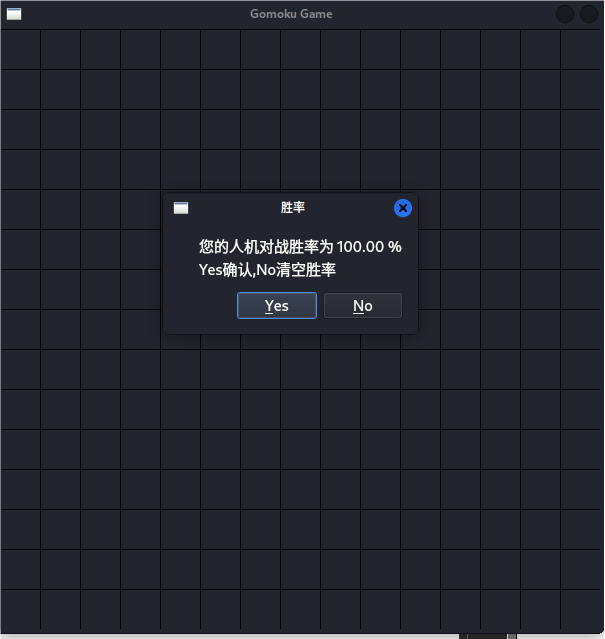
\includegraphics[width=\textwidth]{screenshoot1.png}
        \caption{图1}
        \label{fig:image1}
    \end{subfigure}%
    \hfill
    \begin{subfigure}[b]{0.3\textwidth}
        \centering
        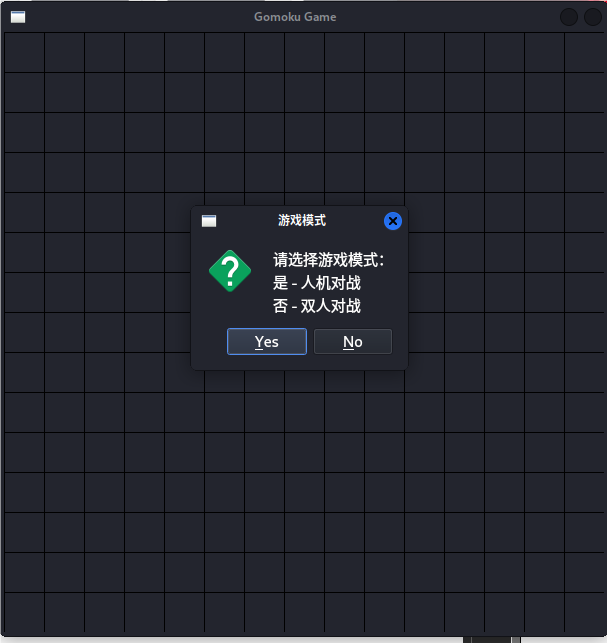
\includegraphics[width=\textwidth]{screenshoot2.png}
        \caption{图2}
        \label{fig:image2}
    \end{subfigure}%
    \hfill
    \begin{subfigure}[b]{0.3\textwidth}
        \centering
        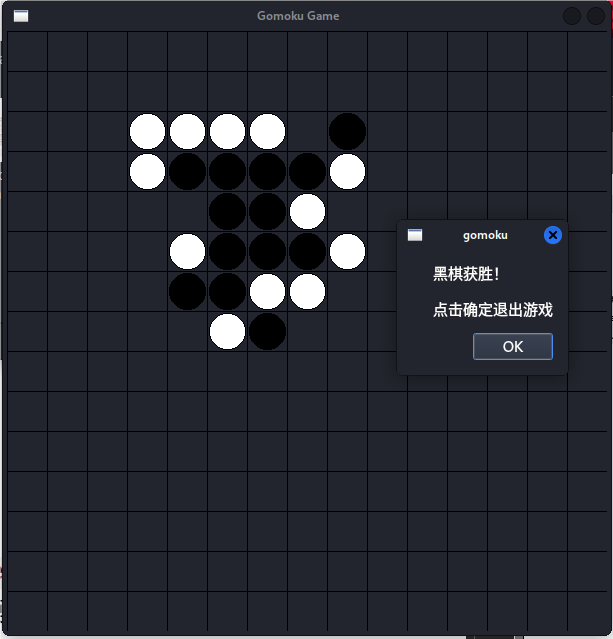
\includegraphics[width=\textwidth]{screenshoot3.png}
        \caption{图3}
        \label{fig:image3}
    \end{subfigure}%
        \hfill
    \begin{subfigure}[b]{0.3\textwidth}
        \centering
        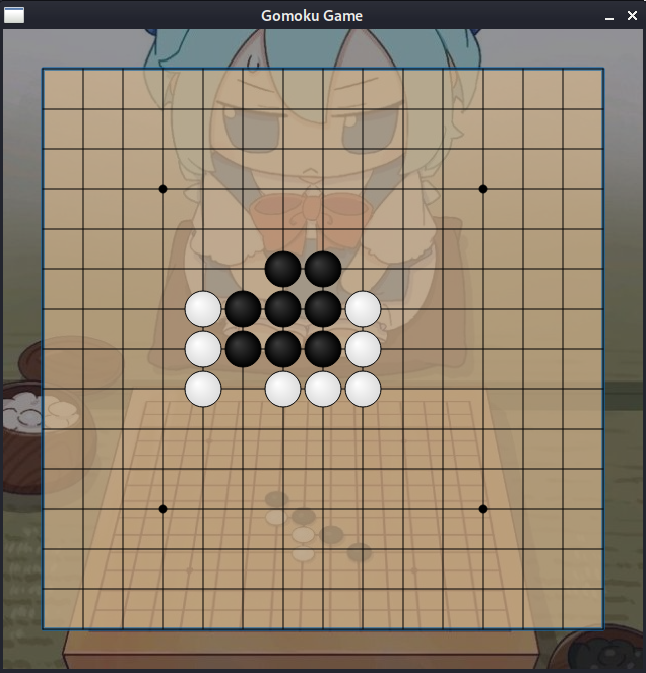
\includegraphics[width=\textwidth]{screenshoot4.png}
        \caption{图4(悔棋前)}
        \label{fig:image4}
    \end{subfigure}%
        \hfill
    \begin{subfigure}[b]{0.3\textwidth}
        \centering
        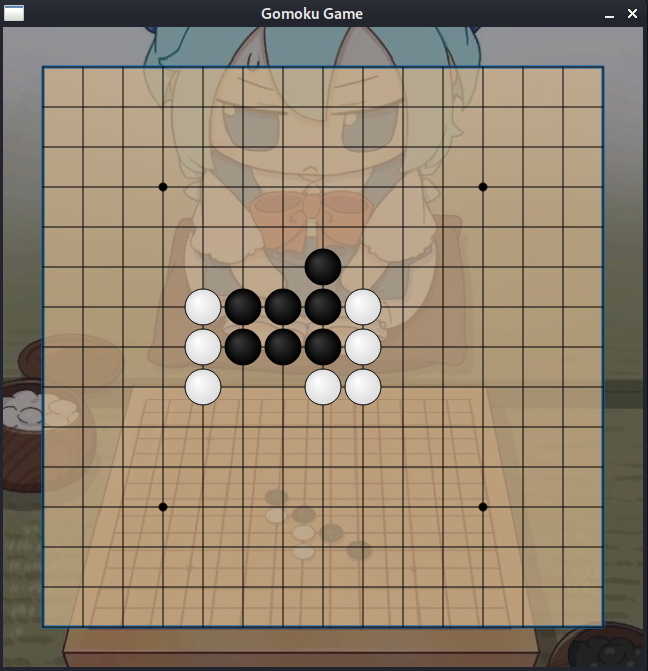
\includegraphics[width=\textwidth]{screenshoot5.png}
        \caption{图5(悔棋后)}
        \label{fig:image5}
    \end{subfigure}
    \caption{测试图例}
    \label{fig:allimages}
\end{figure}

\section{任务分工}
\begin{itemize}
    \item \textbf{2410120028 侯成霖}:负责底层逻辑,算法,界面开发(GomokuBoard, AiPlayer,GameWindow),Latex文档 贡献度60\%
    \item \textbf{2410120036 陶勇豪}:负责文件处理,界面开发(GameWindow,Rating),PPT 贡献度40\%
\end{itemize}

\section{经验总结}
\subsection{遇到的问题与解决}
\begin{itemize}
    \item \textbf{AI只下左上角}:调整分值评估,越在中间的评分越高
    \item \textbf{边界检测错误}:增加边界检查条件
    \item \textbf{显示程序内存溢出}:调整大小加入检查
\end{itemize}

\subsection{改进方向}
\begin{itemize}
    \item 增加难度级别选择
    \item 用栈保留对局信息
    \item 添加音效和动画
    \item 添加黑棋禁手规则,保证公平
    \item 优化AI算法(Minimax+Alpha-Beta剪枝)
\end{itemize}

\subsection{总结体会}
通过本项目,我们深入掌握了:
\begin{itemize}
    \item Qt框架的图形编程技术
    \item linux环境编程操作
    \item 游戏AI设计原则
    \item 面向对象设计模式
    \item 团队协作开发流程
\end{itemize}
	五子棋虽规则简单,但在实现过程中涉及到算法优化、用户体验、代码架构等多方面挑战,是一次宝贵的开发经验。

\end{document}